\documentclass[a4paper,11pt]{article}

\usepackage[spanish]{babel}
\usepackage{multirow}
\usepackage{verbatim}
\usepackage{moreverb}

%Idioma
\usepackage[latin1]{inputenc}
%Letra arial
\usepackage{helvet}
%\renewcommand\familydefault{\sfdefault}
%Para incluir codigo fuente
\usepackage{listings}
%Para tener encabezados y pie de pagina personalizados
\usepackage{fancyhdr}
%Para poner ep�rafe en las imagenes
\usepackage[hang,bf]{caption2}

%------------Gr�ficos------------
%Paquete de gr�ficos
\newif\ifpdf
\ifx\pdfoutput\undefined
	\pdffalse
\else
	\pdfoutput=1
	\pdftrue
\fi

\ifpdf
	\usepackage[pdftex]{graphicx}
	\pdfcompresslevel=9
% 	\pdfcompresslevel=0
	\usepackage{pdfpages}
\else
	\usepackage[dvips]{graphicx}
\fi



% Titulo del Trabajo Practico.
\title{ Trabajo Pr\'actico 0: infraestructura b\'asica   \\
        \Large{ 66.20 Organizaci\'on de las Computadoras } }


% Informaci\'on sobre los autores.
\author{Nicol\'as Calvo, \textit{Padr\'on Nro. 78.914}           	\\
            \texttt{ nicolas.g.calvo@gmail.com }      			\\
            Celeste Maldonado, \textit{Padr\'on Nro. 85.630}              	\\
            \texttt{ maldonado.celeste@gmail.com }                             \\
            Matias Acosta, \textit{Padr\'on Nro. 88.590}                \\
            \texttt{ matiasja@gmail.com }                     		\\
            \LARGE{}         						\\
            \LARGE{}         						\\
            \LARGE{}         						\\
            \Large{2do. Cuatrimestre de 2011}         	\\                       
            \texttt{}         						\\
            \Large{Facultad de Ingenier\'\i{}a, Universidad de Buenos Aires}            \\
       }
\date{}



\begin{document}

\begin{figure}
\centering

\includegraphics[width=100pt]{logofiuba.jpg}
\end{figure}


\maketitle
\thispagestyle{empty}   % quita el numero en la primer pagina
%\renewcommand{\labelenumi}{\alph{enumi}.}


\newpage
% Declaro el indice

\tableofcontents
\newpage

\setcounter{page}{1}

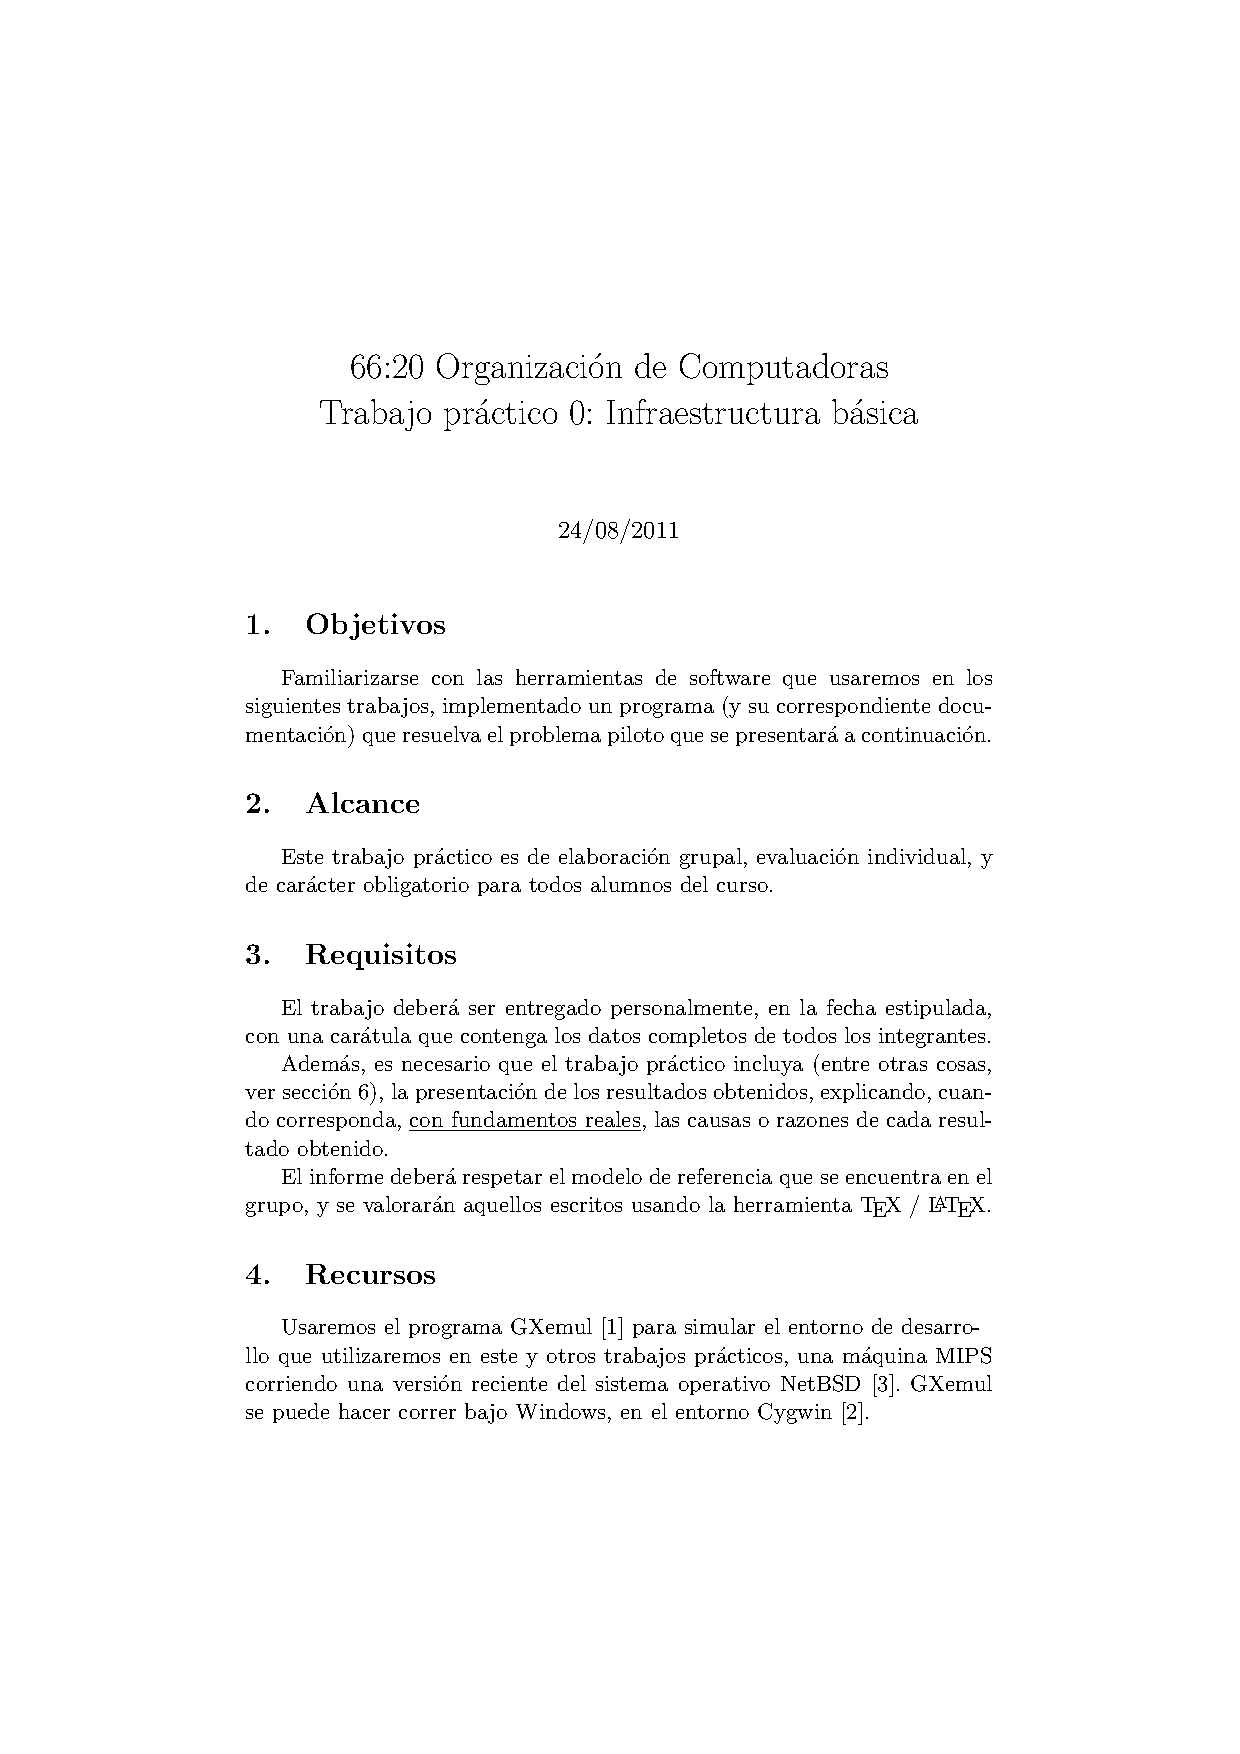
\includepdf[pages={1,2,3},addtotoc={2, section ,1 , Enunciado , Enunciado}]{enunciado.pdf}


\section{Introducci\'on}

Para la realizaci\'on del trabajo pr\'actico fue necesario simular un sistema operativo (NetBSD) que utiliza un procesador MIPS. 
En el simulador utilizamos el programa GXemul, que permite simular el entorno necesario para producir el c\'odigo, compilarlo, 
ejecutarlo y obtener el c\'odigo MIPS32 generado por el compilador.


\section{Programa}

El programa, a escribir en lenguaje C, es una versi\'on minimalista del comando join de UNIX. 
El mismo, realizar\'a la uni\'on de dos archivos seg\'un la primer palabra/campo de cada archivo que ser\'a tomado como 
clave de uni\'on. Si se pasa s\'olo uno de los archivos a unir, se leer\'a de la entrada estandar.

\subsection{Dise�o e implementaci�n}
% falta aca explicar

\paragraph{Proceso y salida}

Primero se verifican los par\'ametros utilizados para llamar el programa. 
En caso de encontrarse un error en alguno de los argumentos de entrada se reporta mediante un mensaje de error.
El formato del archivo de entrada es de texto. 

\paragraph{Manejo de errores}

El manejo de errores se realiza mediante el stream stderr, en caso de error se muestra una leyenda que se corresponde con cada caso.


\subsection{Generaci�n}
Para generar el binario hay que ejecutar el siguiente comando:
\begin{tabbing}
\hspace{3cm}\= 	gcc -Wall -lm -O0 -o tp0 tp0.c\\
\end{tabbing}

Para compilar el c�digo a MIPS se utiliza:

\begin{tabbing}
\hspace{3cm}\= gcc -Wall -O0 -S -mrnames tp0.c\\
\end{tabbing}

\begin{itemize}
\item	Wall: activa todos los mensajes de warning.

\item	O: indica el nivel de optimizacion, en este caso no queremos que el compilador optimice el programa por lo que ponemos nivel 0.

\item	o: genera el archivo de salida.

\end{itemize}

\subsection{Uso y comandos}

\paragraph{}
La entrada del programa ser\'an los dos archivos a unir. En caso de no especificarse uno, el programa leer\'a 
de la entrada estandard stdin.

\paragraph{}
El programa debe tener como salida, la misma informaci\'on que el comando join de UNIX. 
Se debe respetar la presentaci\'on de esta tal cual la realiza el comando. 
Adem\'as el programa debe soportar el orden, cantidad y disposici\'on de los par\'ametros tal cual lo soporta 
el comando original de UNIX. Los mensajes de error deben indicarse via stderr.

\paragraph{}
A continuaci\'on se describen las opciones disponibles:

\begin{itemize}
\item	``-V'' o ``--version'': esta opci\'on muestra la versi\'on del programa. No recibe ning\'un argumento.

\item	``-h'' o ``--help'': esta opci\'on muestra un mensaje de ayuda, el cual posee las opciones que recibe el programa.

\item	``-i'' o ``--ignore-case'': ignora la diferencia en la comparaci\'on de las claves de los archivos.
\end{itemize}


\subsubsection{Ejemplo}


A continuaci\'on se exponen varios ejemplos del uso de la aplicaci\'on. \\

Usamos la opci\'on -h para ver el mensaje de ayuda:
\begin{verbatim}
tp0 -h
Usage: join [OPTION]... FILE1 FILE2
For each pair of input lines with identical join fields, write a line to standard output. The default join field is the first, delimited
by whitespace. When FILE1 or FILE2 (not both) is -, read standard input. \\
-i, --ignore-case ignore differences in case when comparing fields
-h, --help display this help and exit
-v, --version output version information and exit
Important: FILE1 and FILE2 must be sorted on the join fields. \\
E.g., use `sort -k 1b,1' if `join' has no options. \\
Note, comparisons honor the rules specified by ``LC_COLLATE". \\
If the input is not sorted and some lines cannot be joined, a warning message will be given.

\end{verbatim}

Ejemplo de una ejecuci\'on:
\begin{verbatim}
$ cat ApellidoNombre
1 Djokovic, Novak
2 Nadal, Rafael
3 Federer, Roger
4 Murray, Andy
5 Ferrer, David
6 Soderling, Robin
7 Monfils, Gael
8 Fish, Mardy
9 Berdych, Tomas
10 Almagro, Nicolas

$ cat Puntaje
1 13,920
2 11,420
3 8,380
4 6,535
5 4,200
6 4,145
7 3,165
8 2,820
9 2,690
10 2,380

$ tp0 ApellidoNombre Puntaje
1 Djokovic, Novak 13,920
2 Nadal, Rafael 11,420
3 Federer, Roger 8,380
4 Murray, Andy 6,535
5 Ferrer, David 4,200
6 Soderling, Robin 4,145
7 Monfils, Gael 3,165
8 Fish, Mardy 2,820
9 Berdych, Tomas 2,690
10 Almagro, Nicolas 2,380

$

\end{verbatim}

\newpage


\section{Pruebas (Test)}
Se realizaron diferentes pruebas para poder abarcar todos los casos posibles que nos permitan determinar el buen 
funcionamiento del programa.\newline
A continuaci�n se muestran los archivos de prueba y la salida obtenida.

\paragraph[Test1]{Prueba n�1}

Archivo 1: contiene todas las claves sin que esten repetidas ninguna de ellas.
\verbatiminput{../pruebas/in/011}

Archivo 2: contiene todas las claves, en igual forma que en el archivo 1, y estan ordenadas.
\verbatiminput{../pruebas/in/012}


Salida
\verbatiminput{../pruebas/out/1}


\paragraph[Test2]{Prueba n�2}

\label{Test2}
Archivo 1: contiene una clave repetida.
\verbatiminput{../pruebas/in/021}

Archivo 2: contiene todas las claves sin repetir y ordenadas.
\verbatiminput{../pruebas/in/012}

Salida
\verbatiminput{../pruebas/out/2}

\paragraph[Test3]{Prueba n�3}

\label{Test3}
Archivo 1: contiene todas las claves sin que esten repetidas ninguna de ellas.
\verbatiminput{../pruebas/in/011}

Archivo 2: contiene una clave que est� repetida.
\verbatiminput{../pruebas/in/013}

Salida
\verbatiminput{../pruebas/out/3}

\paragraph[Test4]{Prueba n�4}

\label{Test4}
Archivo 1: contiene todas las claves sin que esten repetidas ninguna de ellas.
\verbatiminput{../pruebas/in/011}

Archivo 2: contiene todas las claves sin repetir, pero no est�n ordenadas.
\verbatiminput{../pruebas/in/014}

Salida
\verbatiminput{../pruebas/out/4}

\newpage

\section{C�digo Fuente}
\lstset{language=c,basicstyle=\small,showstringspaces=false,columns=fullflexible,frame=lines,tabsize=4,inputencoding=latin1,extendedchars=true}

\subsection{tp0.c}
% \lstinputlisting{../src/tp0.c}

\subsection{tp0.s}
\lstinputlisting{../assembly/tp0.s}


\newpage

\section{Conclusi�n}
A trav�s del trabajo pr�ctico logramos familizarnos con herramientas del
entorno $Gnu/Linux$. Entre estas herramientas se pueden descatar:  $ssh$ (Secure Shell), $scp$ (Secure Copy),
algunos comandos b�sicos de linux, la utilizaci�n de $pipeline$ para el flujo
de datos y el entorno $netBSD$. 

\end{document}

